%!TEX root = apostila.tex
Na pirâmide de automação, a partir da camada 2, os sistemas utilizados são softwares em computadores, sejam servidores, terminais, desktops, notebooks ou mesmo tablets e smartphones (para o caso do supervisório). No nível de controle, o dispositivo utilizado pode ser um computador, um CLP -- que não deixa de ser um computador -- ou outro dispositivo que incorpora um processador. Hoje em dia até no nível 0 estão ficando cada vez mais comuns os dispositivos ditos \emph{inteligentes}, que incorporam também um microprocessador.

Tais dispositivos digitais abrem espaço para que a comunicação entre eles seja através de um sinal digital, com vantagens em relação a sinais analógicos em imunidade a ruído, possibilidade de redução de custos e de aumento da quantidade de informação, maior facilidade de aplicação de criptografia, entre outras.

Deste modo se conectam os diferentes dispositivos que fazem parte de um sistema de automação através de uma rede de comunicação, de onde vem a importância de entendê-las e estudá-las.

\section{Redes de Comunicação: Introdução e noções básicas}

O problema da comunicação de dados automática entre diversos dispositivos é bastante complexo. Peguemos como exemplo pagar uma conta via internet: é necessária a comunicação do dispositivo caseiro (que seja um tablet) e o computador central do banco (1). Quanto mais rápida for esta comunicação, mais agradável é para o usuário e mais barato é para o usuário e para o banco (2). Obviamente nenhuma das partes envolvidas querem que seja pago o valor errado ou a conta errada (3). Entre o tablet e o servidor do banco estão: o modem wifi, a central telefônica, servidores da companhia telefônica e talvez de outras fornecedoras de serviço (4), e em geral não é do interesse do usuário que a companhia telefônica ou outro elemento saiba de sua senha do banco (5). A comunicação do tablet ao modem é por wifi. Do modem para a central telefônica é pelo fio telefônico. Da central em diante pode ser por cabos de cobre ou, mais provavelmente, por fibra óptica (6). Também, por questão de custos e privacidade, não é desejável que outros elementos recebam aquela informação, mesmo que criptografada (7).

Ou seja, podemos definir, extendendo ao caso geral, que a comunicação de dados envolve:
\begin{enumerate}
	\item transferência de dados de um dispositivo a outro,
	\item em alta velocidade,
	\item sem perda de informação,
	\item passando por dispositivos intermediários,
	\item com privacidade,
	\item envolvendo meios e sistemas de comunicação diferentes,
	\item sem envolver outros dispositivos desnecessariamente.
\end{enumerate}

Claro que há vários casos que não envolvam todos estes aspectos. Pode-se ter comunicações digitais bem mais simples, como no caso de um mouse "conversando" com o computador através da USB, que não requer alta velocidade, nem tem dispositivos intermediários, logo a princípio não requer privacidade nem diferentes meios de comunicação e nem é possível de envolver outros dispositivos. Até mesmo a questão da perda de informação pode não ser necessária em alguns casos, tais como em sistemas VOIP (\emph{Voice Over IP}), onde mais importante que garantir que todos os dados tenham sido recebidos corretamente é manter o atraso da comunicação pequeno o suficiente para não incomodar demais. Mas consideremos inicialmente o caso mais geral.

Para resolver um problema de tal magnitude, foi desenvolvida a idéia de quebrá-lo em várias partes, ou camadas, onde cada camada tem um protocolo responsável por uma determinada parte do problema. A informação fica então passando de camada a camada, acrescida de metadados para resolver todas as questões relativas à comunicação. Tal esquema é também chamado de pilha de protocolos. O chamado modelo OSI foi então criado definindo camadas o mais genéricas possíveis, de modo a abarcar qualquer tipo de comunicação de dados.

\subsection{Modelo OSI}
O modelo OSI (\emph{Open System Interconnection}) é o modelo de referência de redes de dados, criado em 1970 e adotado pela ISO em 1983. Este modelo define 7 camadas de abstração que separam as diferentes tarefas necessárias à comunicação de dados; são as camadas: física, enlace, rede, transporte, sessão, apresentação e aplicação.

\subsubsection{Camada 1 -- Física}
	A camada física é a única que não pode ser implementada em software. Ela lida com as definições eletro-mecânicas necessárias para a comunicação. Ou seja, a camada física define:
	\begin{itemize}
		\item o meio pelo qual os dados são transmitidos -- sinais elétricos por cabo, sinais de rádio, luz, etc;
		\item as características do meio de transmissão, tais como o tipo de cabo, os níveis de tensão, o formato dos conectores, etc;
		\item a taxa de transmissão (tipicamente quantos bits por segundo -- bps).
	\end{itemize}
	Note-se que a taxa de transmissão acaba sendo limitada justamente pelos diversos parâmetros físicos descritos pela camada física de um determinado protocolo de comunicação.

Outro parâmetro definido na camada física é se a rede é \emph{simplex}, \emph{half-duplex} ou \emph{full-duplex}. Simplex significa que a comunicação no meio de transmissão é apenas num sentido (exemplo: televisão), half-duplex é uma comunicação em dois sentidos, mas apenas um por vez (exemplo: walkie-talkie) e full-duplex é uma comunicação em ambos os sentidos ao mesmo tempo (exemplo: telefonia).

A camada física também limita aspectos da chamada topologia da rede, que é a forma como os dispositivos se relacionam entre si, como por exemplo:
\begin{description}
	\item[Ponto-a-ponto] Onde apenas 2 dispositivos se conectam ente si.
	\item[Estrela] Onde um nó central se comunica com os demais nós. Vide sistemas de TV ou rádio.
	\item[Barramento] Onde os vários dispositivos se conectam em paralelo a um único barramento.
	\item[Árvore] Um barramento com derivações.
	\item[Linha] Onde cada dispositivo se conecta diretamente apenas com um ou 2 vizinhos.
	\item[Anel] Uma linha formando um anel.
	\item[Totalmente conectada] Cada dispositivo diretamente conectado a todos os outros da rede.
	\item[Malha] Cada nó conectado a vários outros, sem uma hierarquia ou ordem bem definida.
\end{description}

\subsubsection{Enlace}

A camada de enlace cuida da comunicação de um dispositivo a seu vizinho, que não necessariamente são os pontos inicial e final de uma comunicação.

No exemplo dado acima, do pagamento de conta na internet, esta camada cuida da comunicação entre o tablet e o modem wifi; entre o modem e a central; entre a central e o servidor da companhia telefônica, e assim por diante.

A camada de enlace de um protocolo define:
\begin{itemize}
	\item quem acessa o meio de transmissão e quando,
	\item que sinais indicam o início e o fim de uma transmissão,
	\item mecanismos que detectem e/ou corrijam erros e,
	\item se necessário, para qual dentre vários dispositivos é aquela comunicação específica.
\end{itemize} 

Alguns protocolos de comunicação, tais como USB e ethernet, fazem a conexão ponto a ponto. Neste caso apenas 2 dipositivos podem acessar o meio. Outros sistemas, como o wifi, podem ter vários (em alguns casos, centenas) de dispositivos no mesmo meio. O que torna necessário a definição de quem pode acessar o meio em cada instante. Várias possibilidades existem, entre as quais:
\begin{description}
	\item[mestre-escravo] Neste sistema, a comunicação sempre é iniciada pelo mestre, e um escravo só ocupa o meio quando o mestre requisita uma informação. Ex.: USB, Modbus.
	\item[\emph{token ring}] É passada uma ficha (\emph{token}) virtual entre os dispositivos. Quem tem a ficha pode falar.
	\item[Multiplexação por tempo] Cada dispositivo tem uma hora específica para controlar o barramento. Um sinal periódico (NUT- \emph{Network Update Time}) sincroniza os dispositivos.
	\item[CSMA-CD -- \emph{Carrier Sense Multiple Access with Collision Detection}] Sempre que um dispositivo quer se comunicar com outro, ele checa antes se o meio está livre. Ex.: wi-fi, bluetooth, CAN.
\end{description}

Tipicamente os protocolos da camada de enlace acrescentam uma certa redundância ao dado transmitido, o que permite detectar e até corrigir erros de transmissão. São os chamados códigos corretores de erro, dentre os quais se utiliza bastante o CRC - \emph{Cyclic Redundancy Check}, mas outros são possíveis, desde uma simples checagem de paridade (se há um número ímpar ou par de bits com valor 1), usado nos protocolos de comunicação serial RS232, RS422 e RS485, a códigos convolucionais, usados na ethernet e em redes celulares.

\subsubsection{Rede}
Camada responsável pelo roteamento da informação. Ou seja: Se A quer se comunicar com D, mas A apenas tem ligação direta com B e C, para quem A deve mandar a informação?

Tipicamente este roteamento é feito através de uma tabela que mapeia o endereço lógico de um dispositivo (o endereço usado nas etapas acima, tais como o IP) e o endereço físico, usado pela camada de enlace. Muitos sistemas usam o \emph{MAC address} -- \emph{Medium Access Control Address}, que é um código definido no dispositivo quando de sua fabricação, tipicamente de 48 ou 64 bits, e único para cada dispositivo.

Esta é a última camada a que uma comunicação chega num dispositivo que não o inicial ou final: o programa desta camada checa se o endereço lógico da mensagem é o mesmo daquele dispositivo. Caso contrário, ele busca na tabela de roteamento qual o endereço físico para o qual reenviar aquela mensagem e reenvia, eventualmente através de um dispositivo diferente ou com um protocolo diferente, tal qual mostra a figura \ref{fig:camada_rede}. Isto serve também para fazer a conexão entre diferentes redes.

\begin{figure}[hbt]
	\begin{center}
		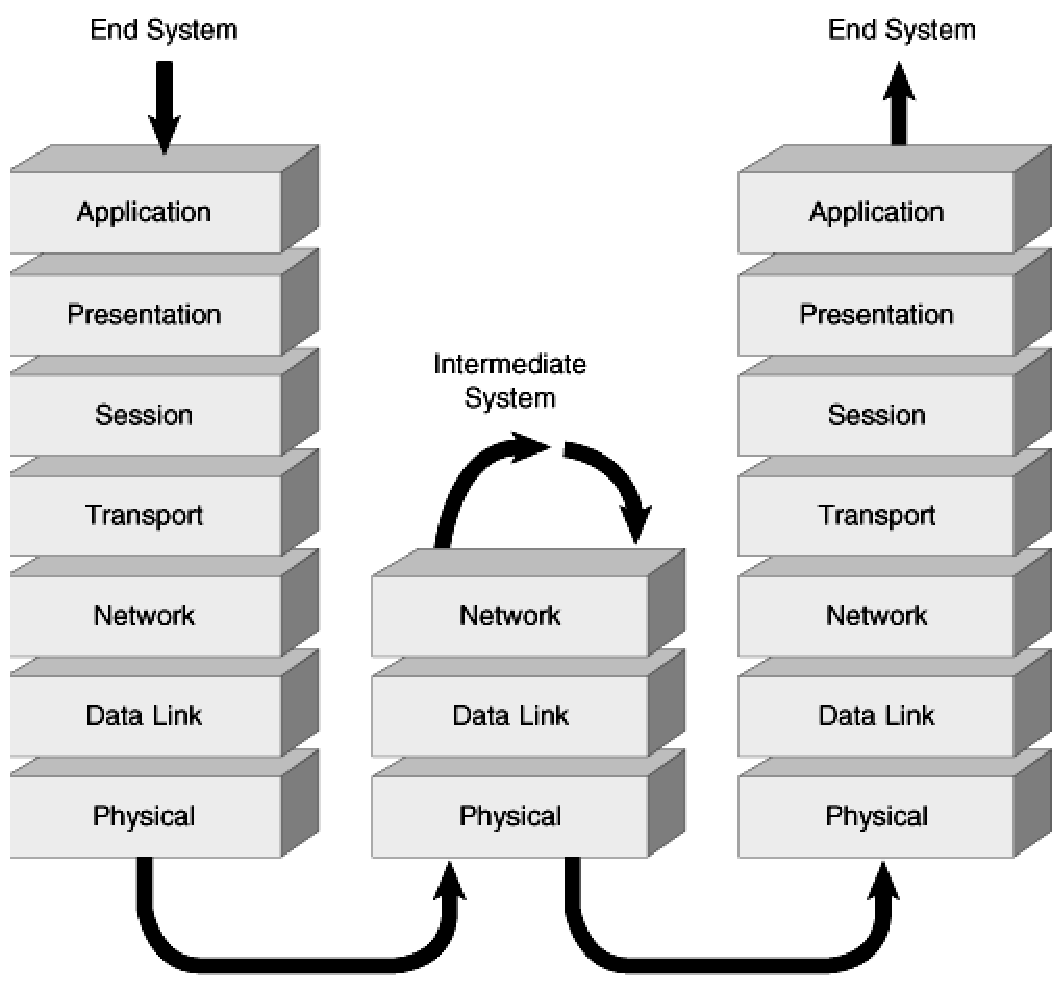
\includegraphics[width=0.6\textwidth]{figuras/network_layer}
	\end{center}
	\caption{Comunicação passando por dispositivo intermediário.}
	\label{fig:camada_rede}
\end{figure}

\subsubsection{Transporte}
 A camada de transporte cuida da comunicação entre o ponto inicial e final.

 São responsabilidades desta camada:
 \begin{itemize}
	 \item garantir a confiabilidade da transmissão, checando se determinado pacote chegou ou não ao destino,
	 \item controlar o fluxo de dados na rede, impedindo de mandar dados de mais que ou sejam mais que o receptor aguente ou que congestionem a rede.
 \end{itemize}
 
 Para melhor ajustar o fluxo de dados, esta camada pode resolver quebrar uma mensagem grande em vários pacotes, mandando um pacote de cada vez para a camada de rede e remontando a mensagem no recebimento. Este é o procedimento usado na transmissão de dados na internet.

 Um conceito interessante utilizado na camada de transporte é o de \emph{Quality of Service -- QoS}, qualidade de serviço. Embora não seja um número único, mas sim a definição de vários parâmetros de uma rede, tais como a ordem de chegada dos pacotes, o atraso na entrega e a falha da entrega de pacotes, a grosso modo pode-se dizer que um alto QoS garante a chegada de todos os pacotes, na ordem em que foram enviados.

 A internet foi originalmente pensada como um sistema de baixo QoS, voltado para a trasnmissão de arquivos. A ordem dos pacotes, a princípio, não interessava e nem o atraso de um pacote. Caso um pacote se perca, simplesmente pede-se que seja reenviado. Uma rede de telefonia, por outro lado, busca garantir que o tempo de cada pacote seja o mesmo, para não piorar a qualidade da voz transmitida.

 Para diversas aplicações industriais, o QoS é importante: não se pode aceitar que uma mensagem de alarme, por exemplo, demore muito a chegar. EtherCAT - \emph{Ethernet for Control Automation Technology} é um exemplo de uma modificação do protocolo Ethernet para mensagens com diferentes QoS.
 
\subsubsection{Sessão}
Esta camada cria, gerencia e termina conexões entre 2 pontos de uma rede. É mais comum na telefonia, onde se gera um caminho fixo para uma determinada ligação. Quando implementada, esta camada gera a tabela que é usada pela camada de rede.

\subsubsection{Apresentação}
Faz a mudança no formato dos dados. Exemplo: troca de quebra de linha entre sistemas Unix e Windows, mudança de codificação windows 1252 para UTF, etc.

Inclue também a criptografia, que é a base para garantir a privaciade da comunicação ponto-a-ponto.

\subsubsection{Aplicação}
A aplicação final, que gera e/ou consome o dado transmitido.

\subsection{Internet}
	A Internet define uma pilha de apenas 4 protocolos: \textbf{enlace}, que engloba também o físico e para o qual há várias possibilidades, tais qual Ethernet, usando par trançado, 802.11, para wi-fi, FC (\emph{Fibre Channel}) 8b/10b para conexões de fibra óptica, entre outros; \textbf{IP} -- \emph{Internet Protocol}, equivalente ao de rede do modelo OSI; \textbf{transporte}, que pode ser um entre vários, sendo o TCP e o UDP os mais comuns e o de aplicação, que envolve sessão, apresentação e aplicação num só, e para o qual existem inúmeros
	.

	A figura \ref{fig:tcp-ip} mostra a sequência que é feita com uma informação passada por http pela internet.
	\begin{figure}[hbt]
		\begin{center}
			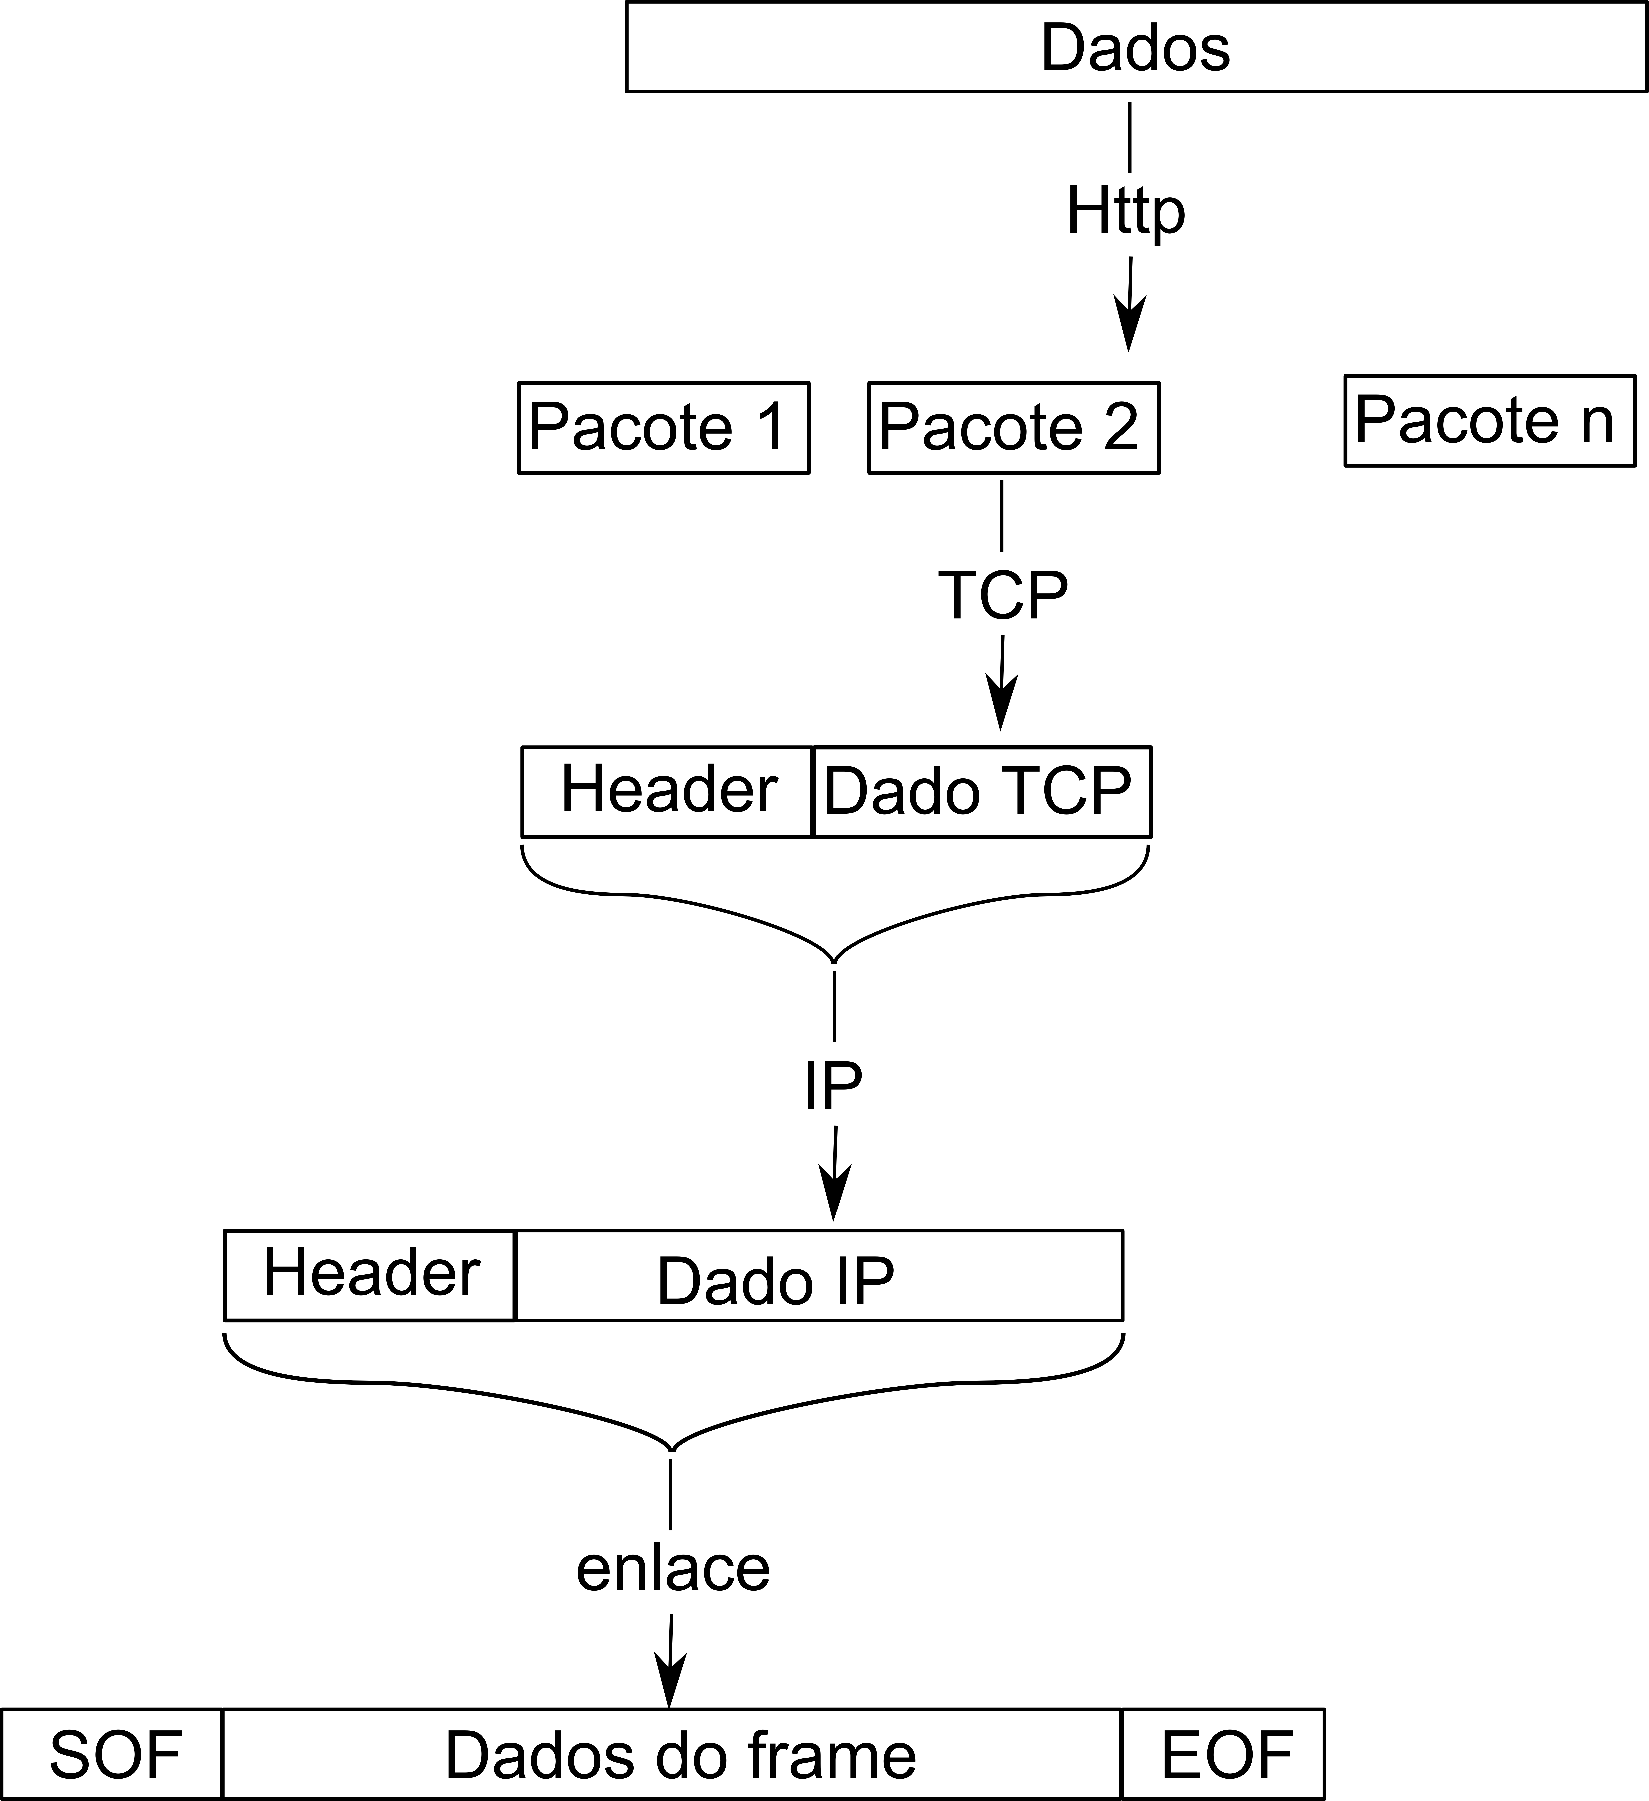
\includegraphics[width=\textwidth]{figuras/tcp-ip}
		\end{center}
		\caption{Encapsulamento da informação na pilha TCP/IP}
		\label{fig:tcp-ip}
	\end{figure}

Como exemplo, um navegador de internet tem vários protocolos do nível de aplicação: http, para buscar páginas não criptografadas, https, para páginas criptografadas, dns, para descobrir o endereço ip relacionado a um determinado endereço, entre outros.

Ao se abrir uma página, tal como a pudim.com.br, o computador primeiramente pega o endereço digitado (\emph{www.pudim.com.br}) e manda uma mensagem ao servidor de dns, que normalmente é definido pelo provedor de acesso, requisitando o endereço IP relativo a este endereço, que no caso é \emph{54.207.20.104}. Ao retornar o endereço, o navegador agora manda uma mensagem tipo \emph{get} pelo protocolo \emph{http} ao IP indicadao pelo servidor DNS e espera um resposta de código 200 do servidor do google, indicando que o que foi pedido existe e contendo a informação pedida, que no caso é o código html da página principal do site.

Este código contém referência a dois arquivos: um arquivo de formatação \verb|estilo.css| e outro de imagem \verb|pudim.jpg|. Cada arquivo deste deve ser pedido por um comando \emph{get} separado.

Toda comunicação neste protocolo é feita usando o protocolo de transporte TCP, que manda cada pacote e espera uma resposta do outro lado. Caso o outro lado não responda ou responda dizendo que teve erro no transporte, o TCP cuida de mandar de novo o pacote para garantir o recebimento do outro lado.

E cada pacote TCP enviado segue pelo protocolo IP (\emph{Internet Protocol}), que pega o endereço IP e através da tabela de roteamento identifica por qual dispositivo de rede (se houver mais de um) e para qual endereço MAC deve mandar aquela informação.